\chapter{谱分析}

\section{目的与操作概要}

分析$\gamma$能谱的目的是通过核素放出的特征$\gamma$\ 能量峰做到核素识别,如果考虑到探测系统的绝对计数效率,也能分析特定堆组件指定位置上的各种核素的含量。

在采谱时,4096道的多道器对应的每一道的计数都保存在多道器中的寄存器里面,停止采谱后,这些计数将保存到磁带上。其中,每一道计数都代表特定的能量间隔,且这个间隔大小是可调。一般实验条件下,一个能量间隔(也称为增益)控制在每道0.3-1.0 keV范围内。换句话说,获得的$\gamma$\ 能谱一般控制在1.2MeV($\sim$\ 0.3$\times$\ 4096)到4MeV(1.0$\times$\ 4096)之间。在一个谱中通过相邻几道的累积计数的增加来确定$\gamma$\ 射线峰(也称为光电峰或全能峰)的存在。实验证明光电峰的计数服从修正高斯曲线。峰的强度由峰高或更多的是高斯曲线峰面积表征。谱中的高斯峰顶点对应的道址即为$\gamma$\ 射线的能量。

$\gamma$\ 能谱分析一般有如下几个步骤:
\begin{enumerate}
\item 确定峰的道址;
\item 判断每个峰是否由统计涨落引起的或是真的光电峰,并且确定峰的起止点;
\item 通过相邻的道判断峰的本底;
\item 高斯曲线拟合峰型;
\item 计算峰面积,扣除对应的本底,即为$\gamma$\ 射线强度的测量值,同时通过高斯曲线的顶点精确定位峰的位置;
\item 查询核数据库,通过道址匹配核素对应的光电峰,确定峰对应的核素;
\item 由核素获得半衰期,$\gamma$\ 射线能量及对应的分支比,以及核素的母体和子体等信息;
\item 一旦核素被确定,计算峰面积即可求出此核素的活度。
\end{enumerate}

分析一个能谱要求探测器系统的效率(即对应的能量响应函数)必须包括需要观察的能量响应范围。同时,在分析过程中,$\gamma$\ 能量和峰道数要精确对应。典型的能谱如图\ref{Fig_4_1}\ 所示。

\begin{figure}
\centering
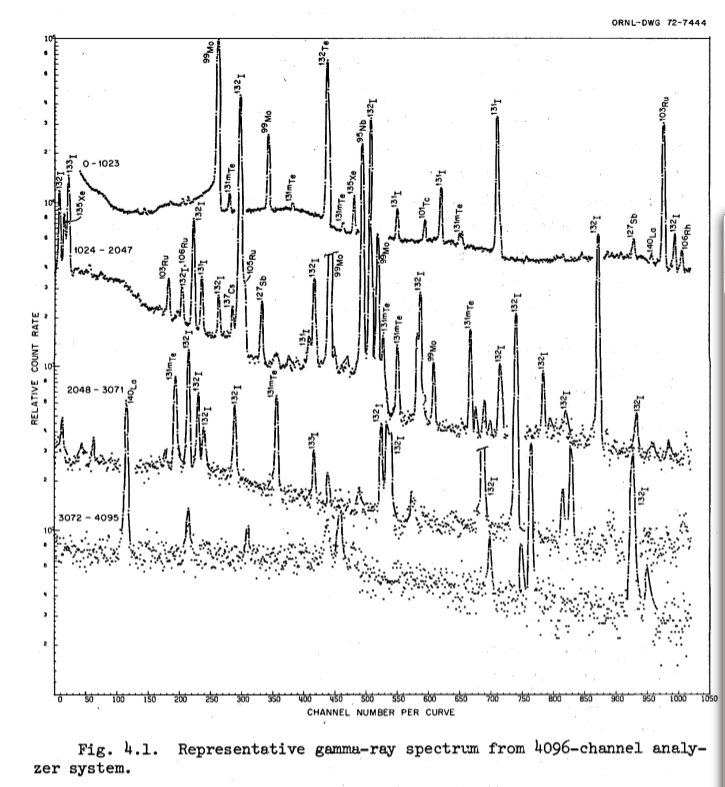
\includegraphics[width=0.8\textwidth]{Fig_4_1}
\caption{Representative gamma-ray spectrum from 4096-channel analyzer system.}
\label{Fig_4_1}
\end{figure}

\section{难点}
在停堆之后,很多短寿命的核素还没来衰变掉,此时采到的能谱里面的很多光电峰重叠在一起,这对增加谱的分析难度。例如,多重峰的起止点难以判断,其本底也无法扣除。重峰拟合主要靠多个高斯曲线左右移动叠加拟合。

如果有一个全面的包括射线能量及对应的分支比的核数据库,我们就能用射线的能量相对容易辨别核素。对于长寿命核素的的数据库比较全,但短寿命的缺少很多。

如上所示,全面地分析一个能谱是很困难,特别是手工解谱。因此,计算机自动化分析谱图将是不可或缺的,特别对于大量谱图而言尤为重要。

\section{同位素表}

本实验花费相当多的精力收集同位素数据。此数据库同时包含了长寿命和短寿命裂变产物的数据,这些数据来源于ORNL核数据项目组收集的最新文献。每个核素列出其$\gamma$\ 射线能量和对应的分支比,并按能量由小到大排列。同时,数据库也给出绝对$\gamma$\ 射线丰度、其前驱和衰变产物。这个表的使用对谱分析有很大的改善。本文给出的数据分析就是基于这张同位素表的。附录A给出了这个基本的同位素表。

以一个可能出错的问题为例,在分析$^{129m}$Te数据时,都会提到。首先这个核素有部分概率衰变到$^{129}$Te再到$^{129}$I,或直接由同核异能素衰变到$^{129}$I。这两种情况下,放出的$\gamma$\ 分支比都十分的小。

这就意味着在活度计算中乘一个大因子而放大了原始光电峰的统计误差。更令人不安的是整个$^{129m}$Te-$^{129}$Te衰变纲图还没有完全确定下来;文献资料提供了几种不同的衰变纲图。由于在$^{129m}$Te衰变中观察第二大光电峰(696.0keV)的同时也有其他核素放出此能量的射线,因此,我们不得不依赖459.6keV峰产生的结果。

基于最新可用的数据,我们评估出$^{129m}$Te衰变到$^{129}$Te再到$^{129}$I放射出459.6keV的分支比为4.9\%。不过随后提交的评估结果更为准确。$^{129}$Te衰变到$^{129}$I放射出459.6keV的分支比为7.7\%.

\section{计算机程序}

如前所述,计算机必须能正确处理本实验要分析的数据。现在最主要的问题是哪里能找到一个能分析存在多重峰的谱的程序。实验采得的谱的复杂程度为每个谱估计有150到230个峰。

ORNL数学部门开发了一个高效的$\gamma$能谱分析程序——GAMSPEC-3,但此程序不具备多重峰分析能力,且只能分析单峰不超过75个的能谱,也不能辨别核素类别。这些不足限制了很多谱的分析,尤其对存在短寿命核素的能谱。Gunnink\footnote{R. Gunnink et al., Identification and Determination of Gamma Emitters by Computer Analysis of Ge(Li) Spectra, LRL-UCID-15140.}等人开发了能满足本实验要求的多功能$\gamma$能谱分析程序——GAMANAl。此程序在劳伦斯放射性实验室(LRL)的CDC-6600计算机上用FORTRAN语言开发而来,又被阿贡实验室(ANL)的N.D.Dudey等人用FORTRAN-IV语言移植到IBM-360系列计算机上。通过ORNL数学部门的能力,此程序也在ORNL的计算机上正常运行。此程序花了LRL近五年的开发时间,ANL用两年时间移植到IBM-360计算机上,而ORNL用了4个月。

此程序实现峰定位(单峰、二重峰和三重峰)和通过峰位实现大量核素的辨别和计算。它能处理400个单峰,100个二重峰和100个三重峰。虽然此程序源于Gunnink,但本实验室做了一些改进,使它支持本实验室的核素数据库。例如源程序是读入一个多项式的系数作为整个探测系统的效率曲线,而本实验室改为用多对能量-效率曲线点就能自动得出相应的效率曲线。通常可支持60对能量-效率曲线点。为了减少纸张浪费,可用堆不同表格做不同的输出格式变化。

虽然此程序满足本实验大部分谱的分析工作,但依然存在一些问题:
\begin{enumerate}
\item{在一些特别的能量范围里,很多峰叠加在一起。此程序只能分析到3重峰,对于三重峰以上的就显得无能为力。}
\item{谱中短寿命核素太多,但核数据库又没有足够的信息,此种谱一般不做分析。}
\item{除非记录了所有核素的详细的衰变链,否则,当通过不同辨别测试方法,程序有时会由于找不到母体和子体而拒绝鉴别。唯一的方法是在能量库中分离母子体关系。例如,95衰变链中,$^{95}$Nb被分离出来而$^{95}$Zr依然在熔盐里。只要$^{95}$Zr作为母体,$^{95}$Nb在此程序中将无法鉴别。当然,这与程序的性能无关。}
\end{enumerate}
